\documentclass[a4paper,12pt]{journal}
\usepackage[dvipsnames, svgnames, x11names]{xcolor} 
\usepackage{amsmath}
\usepackage{amssymb}
\usepackage[margin=2.5cm]{geometry}
\usepackage{graphics}
\usepackage{ulem}
\usepackage{setspace}
\usepackage{listings}
\usepackage{algorithm}  
\usepackage{algpseudocode}  
\usepackage{amsmath}  
\usepackage{xcolor}
\usepackage[greek,english]{babel}
\usepackage{chemformula}
\usepackage{wrapfig}
\usepackage{multirow}
\usepackage{booktabs}
\usepackage{fancyhdr}
\usepackage{pgfplots}
\usepackage{tikz}
\pagestyle{fancy}
\usetikzlibrary{math}
\rmfamily
\fancyhf{}
\fancyfoot[R]{\thepage}
\fancyhead[R]{VG441 HW2}
\title{VG441 Problem Set 2}
\author{Anna Li \\Student ID: 518370910048}
\date{\today}
\lstset{
	columns=fixed,     
	numbers=left,                                        % 在左侧显示行号
	numberstyle=\tiny\color{gray},                       % 设定行号格式
	frame=none,                                          % 不显示背景边框
	backgroundcolor=\color[RGB]{245,245,244},            % 设定背景颜色
	keywordstyle=\color[RGB]{40,40,255},                 % 设定关键字颜色
	numberstyle=\footnotesize\color{darkgray},           
	commentstyle=\it\color[RGB]{0,96,96},                % 设置代码注释的格式
	stringstyle=\ttfamily\slshape\color[RGB]{128,0,0},   % 设置字符串格式
	showstringspaces=false,                              % 不显示字符串中的空格                                        % 设置语言
}
\begin{document}
	\maketitle
	\section*{Problem 1}
	From the question, we could conclude that 
	\begin{equation}
		\begin{array}{r c l}
			\lambda&=& 500\text{ tons/day}\\
			K&=& 2250\text{ per order}\\
			i&=&0.25/365\text{ per day}
		\end{array}\\
	c=\left\{
	\begin{array}{l l}
		\$1490\text{ per ton}, &Q<1200\\\
		\$1220\text{ per ton}, &1200\leq Q<2400\\
		\$1100\text{ per ton}, &Q\geq 2400\\
		\end{array}\right.
	\end{equation}
\subsection*{All-Units Discount}
For this structure, we could generate the $g(Q)$, and get that:
\begin{equation}
	\begin{array}{r c l}
		g_0(Q)&=&1490*500+2250*500/Q+0.25/365*1490/2*Q\\
		g_1(Q)&=&1220*500+2250*500/Q+0.25/365*1220/2*Q\\
		g_2(Q)&=&1100*500+2250*500/Q+0.25/365*1100/2*Q\\
	\end{array}
\end{equation}
And we could draw the graph like:
\begin{figure}[h]
	\begin{tikzpicture}
		
		\begin{axis}[
			axis x line=middle,
			axis y line=middle,
			ylabel=$g(Q)$,
			xlabel=$Q$
			]
			\addplot[domain=0:1200]{745000+1125000/x+0.51*x};
			\addplot[domain=1200:2400]{610000+1125000/x+0.418*x};
			\addplot[domain=2400:3600]{550000+1125000/x+0.377*x};
		\end{axis}
	\end{tikzpicture}
	\caption{Total cost for all-units quantity discount structure}
\end{figure}
and the $Q_j^\ast$ is:
\begin{equation}
	\begin{array}{r c l}
		Q_0^\ast&=&1484.8\\
		Q_1^\ast&=&1640.9\\
		Q_2^\ast&=&1728.1\\
	\end{array}
\end{equation}
Among these value, $Q_1^\ast$ is feasible, which is:
$$g_1(1640.9)=611371$$
Then we caculare the cost of breakpoints to the right of $Q_1^\ast$and get:\\
$$g_2(2400)=551372$$
Therefore, the optimal orfer quantity is $Q=2400$, which incurs a purchase cost of 1100 and a total daily cost pf \$551372
\subsection*{Incremental Discount}
For this instructure, we could calculate that :
\begin{equation}
	\begin{array}{r c l}
		\bar{c_1}&=&1490*1200-1220*1200=324000\\
		\bar{c_2}&=&1490*1200+1220*1200-1100*2400=612000\\
	g_0(Q)&=&1490*500+2250*500/Q+0.25/365*1490/2*Q\\
	g_1(Q)&=&1220*500+0.25/365*324000/2+(2250+324000)*500/Q+0.25/365*1220/2*Q\\
	g_2(Q)&=&1100*500+0.25/365*612000/2+(2250+612000)*500/Q+0.25/365*1100/2*Q\\
	\end{array}
\end{equation}
And we could draw the graph like:
\begin{figure}[h]
	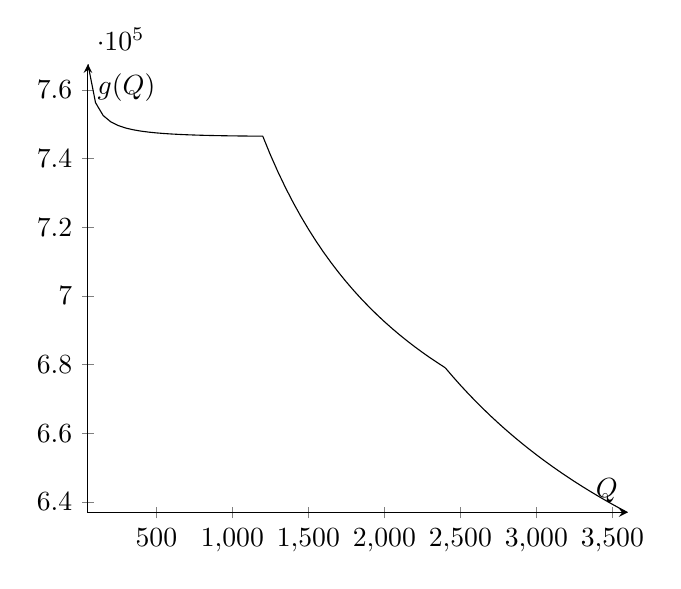
\begin{tikzpicture}
		
		\begin{axis}[
			axis x line=middle,
			axis y line=middle,
			ylabel=$g(Q)$,
			xlabel=$Q$
			]
			\addplot[domain=0:1200]{745000+1125000/x+0.51*x};
			\addplot[domain=1200:2400]{610111+163125000/x+0.418*x};
			\addplot[domain=2400:3600]{550210+307125000/x+0.377*x};
		\end{axis}
	\end{tikzpicture}
	\caption{Total cost for incremental discount structure}
\end{figure}
Next, we caculate the $Q_j^\ast$ for each j:
\begin{equation}
	\begin{array}{r c l}
		Q_0^\ast&=&1484.8\\
		Q_1^\ast&=&19759.3\\
		Q_2^\ast&=&28553\\
	\end{array}
\end{equation}
Therefore, only $Q_2^\ast$ is available.
$$g_2(28553)=571722.169$$
SInce there are no breakpoints to the right, therefore, the optimal order quantity if $Q=28553$, which incurs a total amount daily cost is \$571722
\end{document}
